\documentclass{beamer}

%
% Choose how your presentation looks.
%
% For more themes, color themes and font themes, see:
% http://deic.uab.es/~iblanes/beamer_gallery/index_by_theme.html
%
\mode<presentation>
{
  \usetheme{Warsaw}       % or try Darmstadt, Madrid, Dresden, ...
  \usecolortheme{default} % or try albatross, beaver, crane, ...
  \usefonttheme{default}  % or try serif, structurebold, ...
  \setbeamertemplate{navigation symbols}{}
  \setbeamertemplate{caption}[numbered]
} 

\usepackage[greek]{babel}
\usepackage[utf8]{inputenc}

\title{Αφιέρωμα στο νεκροταφείο του Γκέτισμπουργκ}
\author{Αβραάμ Λίνκολν}
\institute{Ηνωμένες Πολιτείες Αμερικής}
\date{19 Νοεμβρίου 1863}

\begin{document}

\begin{frame}
  \titlepage
\end{frame}

\begin{frame}{Περιγραφή}
  \tableofcontents
\end{frame}

\section{Ατζέντα}

\begin{frame}{Ατζέντα}

\begin{itemize}
  \item  Συναντήθηκαν στο πεδίο της μάχης (υπέροχο)
  \item Αφιερώστε τμήμα του πεδίου
  \item Ημιτελή έργα (εξαιρετικές αποστολές)
\end{itemize}

\end{frame}

\begin{frame}{Όχι στην ατζέντα!}

\begin{itemize}[<+->]
  \item Αφιερώστε
  \item Τιμείστε 
  \item Προσθέστε ή μειώστε
  \item Σημειώστε ή θυμηθείτε τι λέμε
\end{itemize}

\end{frame}

\section{Ανασκόπηση}

\begin{frame}{Βασικοί Στόχοι \& Παράγοντες Επιτυχίας}

\begin{itemize}
\item Τι κάνει το έθνος μοναδικό:
  \begin{itemize}
    \item \textlatin{Conceived in Liberty}
    \item ισότητα
  \end{itemize}
\end{itemize}

\begin{block}{Κοινό όραμα:}
\begin{itemize}
\item Η νέα γέννηση της ελευθερίας
\item Κυβέρνηση για/από τον λαό.
\end{itemize}
\end{block}

\end{frame}

\begin{frame}{Οργανωτική Επισκόπηση}

\begin{figure}
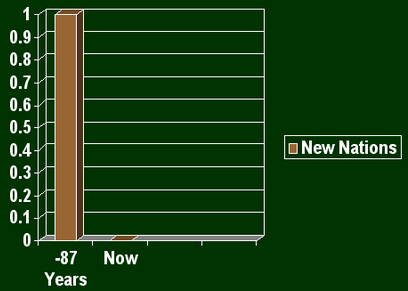
\includegraphics[width=0.5\textwidth]{gettysburg_graph}
\end{figure}

\begin{block}{\textlatin{Four Score and Seven}}
\begin{equation}
-(4 \times 20 + 7) = -87
\end{equation}
\end{block}

\end{frame}

\section{Σύνοψη}

\begin{frame}{Σύνοψη}

\begin{columns}
\begin{column}{0.4\textwidth}
\begin{itemize}
\item Νέο έθνος
\item Εμφύλιος πόλεμος
\item Πεδίο αφιέρωσης
\end{itemize}
\end{column}
\begin{column}{0.6\textwidth}
\begin{itemize}
\item Αφιερωμένο σε ημιτελή έργα
\item Η νέα γέννηση της ελευθερίας
\item Η κυβέρνηση να μην χαθεί
\end{itemize}
\end{column}
\end{columns}

\end{frame}

\end{document}
